\section{Zusammenführung des Actor-Critic-Verfahrens}
\label{sec:Synthesis_Actor_Critic}

Im vorherigen Kapitel haben wir eine Trainingsumgebung für verstärkendes Lernen etabliert, die das Sammeln von Zuständen, Aktionen und Belohnungen (Rewards) umfasst. Diese Daten werden in einem Replay Buffer gespeichert, aus dem sie entsprechend der Batch-Größe  für das Training entnommen werden.(siehe Abschnitt \ref{sec: Batch})

\paragraph{Die Dynamik des Replay Buffers}
Aus dem Replay Buffer (siehe Abschnitt  \ref{sec:Replay Buffers}) werden Datensätze extrahiert, die simultan zur Berechnung des Gradienten und zur Aktualisierung der Actor-Critic Architektur herangezogen werden.
Der Replay Buffer ist das Herzstück unserer Trainingsdynamik. Er speichert die Erfahrungen, die der Algorithmus im Laufe der Simulation macht, und ermöglicht es uns, die komplexen Zusammenhänge zwischen Aktionen und resultierenden Belohnungen zu extrahieren.

\paragraph{Die Aufgabe des Critics}
Der Critic bewertet die vom Actor ausgeführte Policy und den gegebenen Zustand,evaluiert die Effektivität der vom Actor vorgeschlagenen Aktionen im Kontext der Schaltung ( siehe Abschnitt \ref{eq:critick update}). Die generierten Schätzwerte des Critics werden mit den tatsächlichen Belohnungen verglichen, womit der Critic das Verhalten der Schaltung in Abhängigkeit von der jeweiligen Konfiguration prognostiziert. Der Critic  Durch das Abgleichen seiner Vorhersagen mit den tatsächlichen Belohnungen lernt der Critic, das Verhalten der Schaltung präzise vorherzusagen und unterstützt damit die zielgerichtete Anpassung der PID-Koeffizienten.

\paragraph{Optimierungsmechanismus des Actors}
Die Feinjustierung des Actors ist ein zentraler Bestandteil des Lernprozesses innerhalb der Actor-Critic Architektur. Anstatt komplexe Bewertungen vorzunehmen, wird ein Gradient berechnet, der die Gewichte des Actors so anpasst, dass die Schätzung des Critics in die richtige Richtung gelenkt wird, um den Reward zu maximieren (siehe Abschnitt \ref{eq:actor update}). Dieser Ansatz ermöglicht es dem Actor, aus den Prognosen des Critics zu lernen und seine Policy systematisch so zu verfeinern, dass die Belohnungsausschüttung erhöht wird. Es handelt sich hierbei um den Kern des Lernvorgangs, bei dem der Actor durch die Adjustierung seiner Gewichte basierend auf der Kritik und den Belohnungen iterativ verbessert wird.

\begin{figure}[htbp]
    \centering
		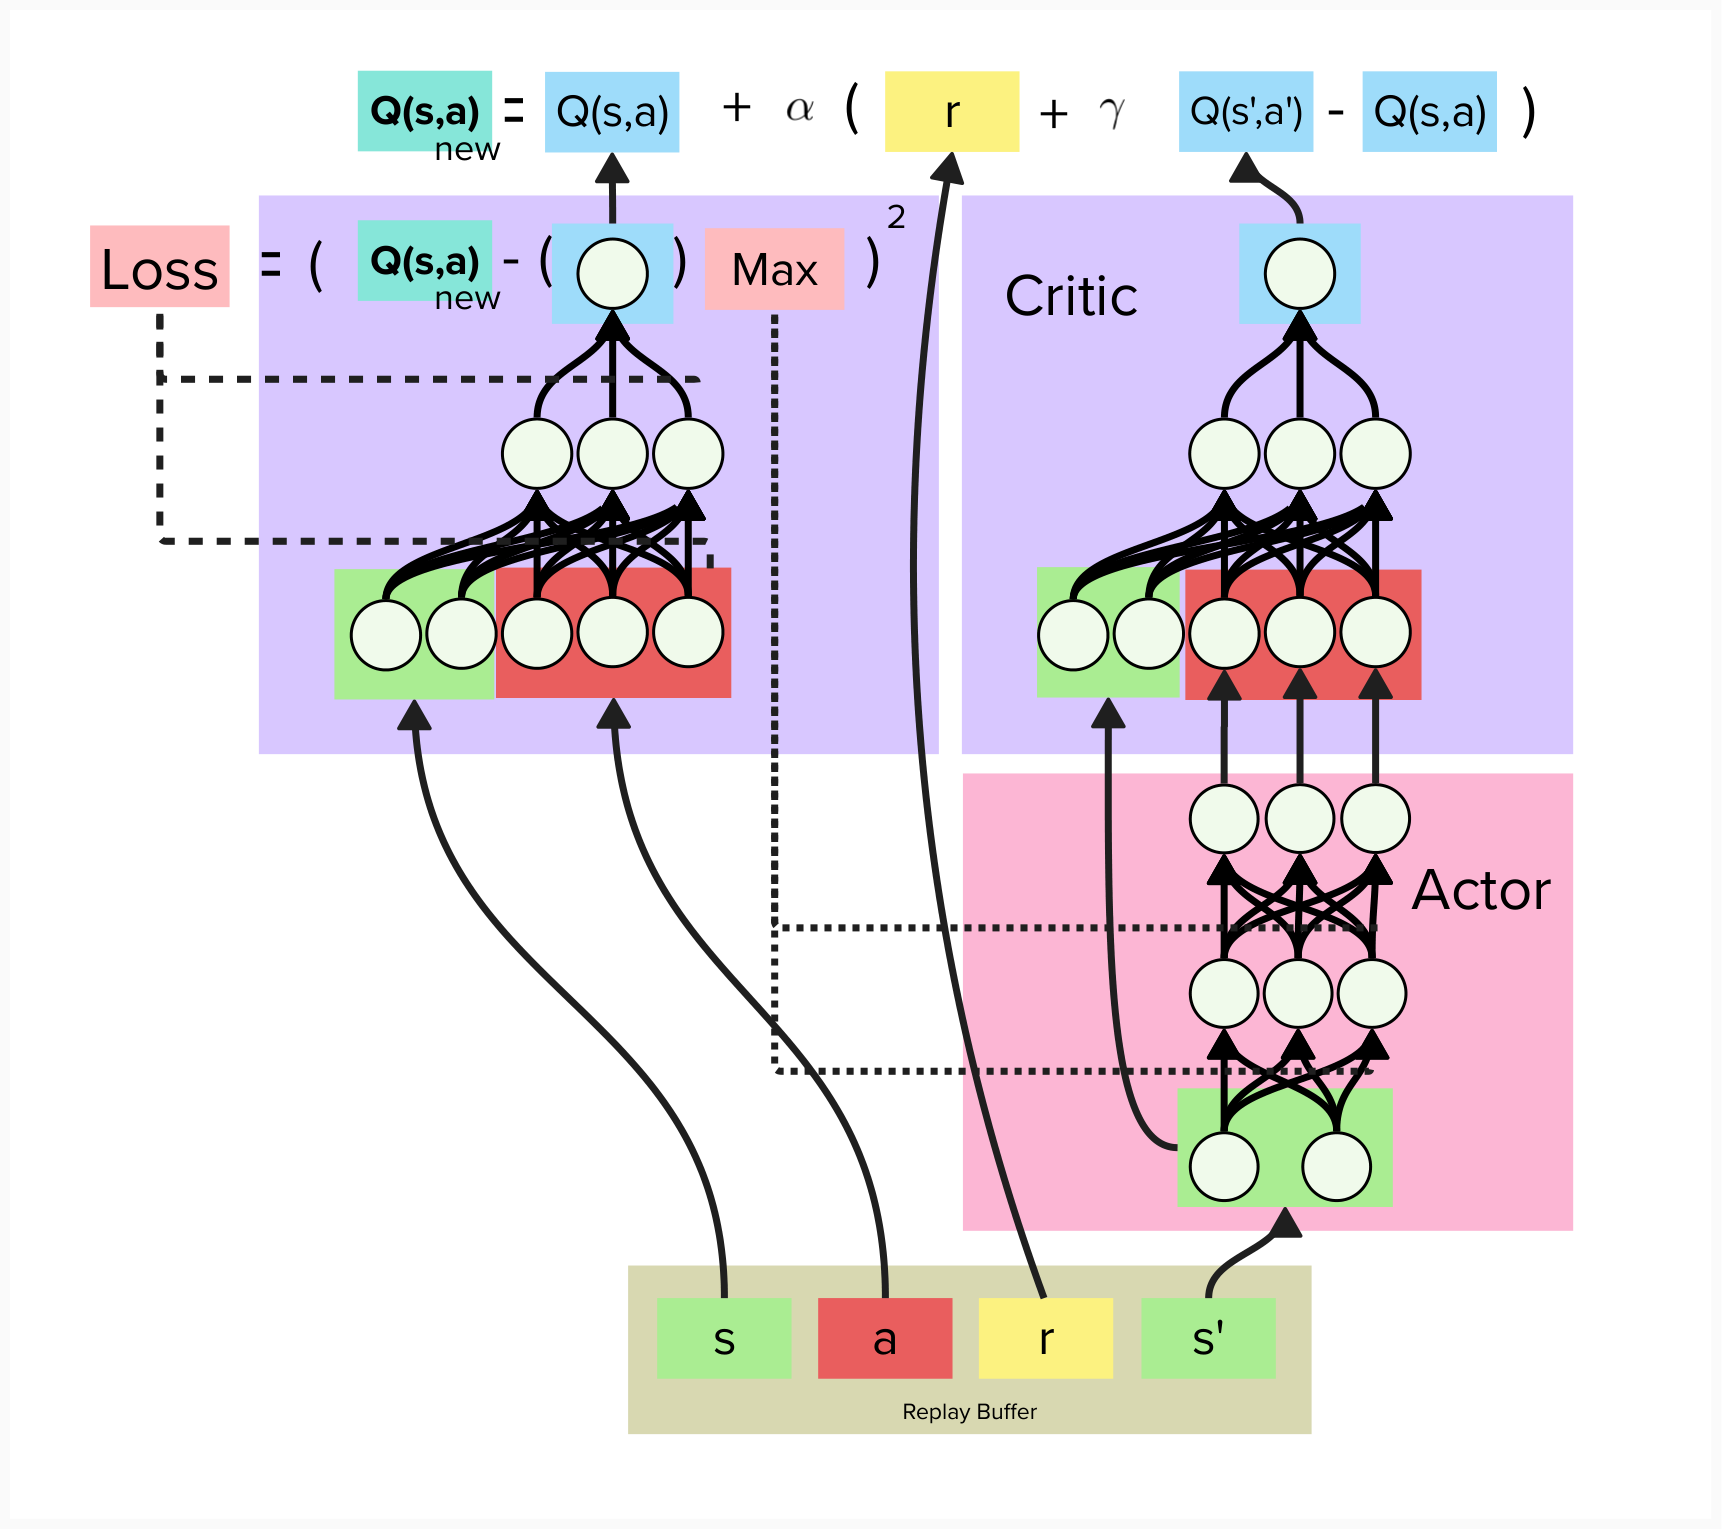
\includegraphics[width=\linewidth, trim=10px 10px 10px 10px, clip]{3Experiment/2Experiment/5Actor_Critick.png}
    \caption{Zusammengefasste Visualisierung des Update-Prozesses in der Actor-Critic Architektur.}
    \label{fig:ActorCriticSynthesis}
\end{figure}


\paragraph{Kontinuierliche Verbesserung durch Training}
Die stetige Aktualisierung des Gradienten nach jedem Simulationsschritt sorgt für eine kontinuierliche Anpassung und Verfeinerung der Actor-Critic Architektur (siehe Abschnitt \ref{sec:Synthesis_Actor_Critic}), was die Belohnungen im Laufe der Zeit maximiert. Angenommen, das Ziel ist eine direkte Optimierung der Belohnungen in unserer Simulation – die Herausforderung besteht darin, dass die komplexe Pipeline von Aktionen bis hin zum endgültigen Reward nicht mit einfachen mathematischen Mitteln abgebildet werden kann. Daher nutzen wir den Actor-Critic Ansatz, um einen einfacheren Gradienten in Bezug auf den erwarteten Reward zu maximieren, was indirekt die Optimierung der Aktionen ermöglicht.


 
